% metadata.tex
\def\documentTitle{Preliminary Design Report}
\def\documentTeam{CDOSR (CoderDojo Oradea Space Robotics)}
\def\documentOrganization{CoderDojo Oradea}
\def\documentCountry{Romania}
\def\documentVersion{1.0}
\def\documentDate{\today}
\def\documentCompetition{Romanian CanSat Competition 2025}
% Define all input paths
\makeatletter
\def\input@path{%
  {./styles/}%
  {./content/appendices/}%
  {./content/sections/}%
  {./content/sections/section_1/}%
  {./content/sections/section_2/}%
  {./content/sections/section_4/}%
  {./content/sections/section_5/}%
  {./content/sections/section_6/}%
  {./content/sections/section_7/}%
}
\makeatother

% Define commands for importing from specific sections
\newcommand{\inputSectionOne}[1]{\input{./content/sections/section_1/#1}}
\newcommand{\inputSectionTwo}[1]{\input{./content/sections/section_2/#1}}
\newcommand{\inputSectionThree}[1]{\input{./content/sections/section_3/#1}}
\newcommand{\inputSectionFour}[1]{\input{./content/sections/section_4/#1}}
\newcommand{\inputSectionFive}[1]{\input{./content/sections/section_5/#1}}
\newcommand{\inputSectionSix}[1]{\input{./content/sections/section_6/#1}}
\newcommand{\inputSectionSeven}[1]{\input{./content/sections/section_7/#1}}
\newcommand{\inputAppendix}[1]{\input{./content/appendices/#1}}

\documentclass[11pt]{article}
\usepackage{CDOSR_CanSat}

% document_settings.tex
% Document-specific settings
\setlength{\headheight}{36.58205pt}
\addtolength{\topmargin}{-24.58205pt}

% Set desired section numbering depth
\setcounter{secnumdepth}{3}
\setcounter{tocdepth}{3}

% Set up headers and footers
\fancyhf{}
\fancyhead[L,R]{\thepage}
\fancyhead[R]{\textbf{\leftmark}}
\fancyhead[LO]{\textbf{\rightmark}}

% Set default image paths
\graphicspath{{images/}{images/template/}{images/diagrams/}{images/photos/}{icons/}{images/cdr/}{images/pdr/}}

% Additional packages for the enhanced branding manual
\usepackage{xcolor}
\usepackage{tikz}
\usetikzlibrary{calc}
% \usepackage[skins,breakable]{tcolorbox}
\usepackage{listings}
\usepackage{booktabs}
\usepackage{multicol}
\usepackage{enumitem}
\usepackage{fontawesome5}
\usepackage{graphicx}
\usepackage{calc}
\usepackage{tabularx}

% Define the CDOSR colors from the color palette
\definecolor{CDOSRPrimary}{RGB}{0, 103, 149}     % DeepSkyBlue4 #006795
\definecolor{CDOSRSecondary}{RGB}{224, 246, 253} % LightCyan1 #e0f6fd
\definecolor{CDOSRAccent}{RGB}{192, 0, 0}        % Red #c00000
\definecolor{CDOSRText}{RGB}{51, 51, 51}         % Dark gray #333333
\definecolor{CDOSRBackground}{RGB}{242, 242, 242} % Light gray #f2f2f2
\definecolor{CDOSRBlack}{RGB}{0, 0, 0}            % Black #000000
\definecolor{CDOSROrange}{RGB}{255, 140, 0}       % Orange #ff8c00
\definecolor{CDOSRDarkRed}{RGB}{178, 34, 34}      % FireBrick #b22222
\definecolor{CDOSRWhite}{RGB}{255, 255, 255}      % White #ffffff

% Color swatch command with all values
\newcommand{\colorswatch}[6]{%
\begin{tcolorbox}[
  colback=#1,
  colframe=black,
  coltext=#2,
  width=0.95\linewidth,
  arc=0mm,
  boxrule=0.5pt
]
  \textbf{#3}\\
  RGB: #4\\
  CMYK: #6\\
  HEX: \#\texttt{#5}\\
  Name: \texttt{#1}
\end{tcolorbox}
}

% Typography sample command with enhanced details
\newcommand{\fontsample}[3]{%
\begin{tcolorbox}[
  colback=white,
  colframe=CDOSRPrimary,
  width=0.95\linewidth,
  arc=2mm,
  boxrule=0.5pt
]
  \textbf{#1}\\
  #2\\
  \vspace{0.3cm}
  {\fontfamily{#3}\selectfont
  ABCDEFGHIJKLMNOPQRSTUVWXYZ\\
  abcdefghijklmnopqrstuvwxyz\\
  0123456789
  }\\
  \textbf{Technical Details:}\\
  Font Family: #3\\
  Line Height: 1.2 - 1.5× font size\\
  Tracking: Normal (0)
\end{tcolorbox}
}

% Command for displaying incorrect examples
\newcommand{\badexample}[2]{%
\begin{tcolorbox}[
  colback=CDOSRBackground,
  colframe=CDOSRAccent,
  title={\textbf{INCORRECT: #1}},
  width=0.95\linewidth,
  arc=2mm,
  boxrule=0.5pt
]
#2
\end{tcolorbox}
}

% Command for displaying color combinations
\newcommand{\colorcombination}[5]{%
\begin{tcolorbox}[
  colback=#1,
  colframe=#2,
  coltext=#3,
  title={\textbf{#4}},
  title colback=#2,
  title colframe=#2,
  title coltext=white,
  width=0.95\linewidth,
  arc=2mm,
  boxrule=0.5pt
]
#5
\end{tcolorbox}
}

\title{CoderDojo Oradea Space Robotics\\Enhanced Branding Manual}
\author{CDOSR Team}
\date{\today}

\begin{document}

\cansattitle{Enhanced Branding Manual}{img_CDOSR.png}{img_CANSAT_RO.png}

\newpage
\tableofcontents
\pagestyle{plain}

\newpage
\section{Introduction}

This enhanced branding manual establishes the official visual identity for CoderDojo Oradea Space Robotics (CDOSR). Consistent use of these brand elements will help build recognition and credibility for our team as we participate in the CanSat competition and related space technology programs.

The CDOSR team represents CoderDojo Oradea in space and robotics technologies, specifically focusing on CanSat competitions. Our visual identity reflects our commitment to education, innovation, and excellence in space science.

This document provides comprehensive guidelines for the use of our logo, colors, typography, and document templates. Following these standards ensures that all materials produced by or for CDOSR maintain a consistent, professional appearance that reinforces our brand identity.

\section{Logo}

\subsection{Primary Logo}

The CDOSR primary logo represents our team's identity and should be used as the main visual identifier on all official communications and materials.

\begin{figure}[h]
    \centering
    
\includegraphics[width=4cm]{img_CDOSR.png}
    \caption{\small{CDOSR Primary Logo}}
    \label{fig:primary-logo}
\end{figure}

\subsection{Secondary Logos}

In addition to our primary logo, CDOSR uses the Romanian CanSat Competition logo as a secondary visual element, especially in competition documentation.

\begin{figure}[h]
    \centering
    
\includegraphics[width=4cm]{img_CANSAT_RO.png}
    \caption{\small{Romanian CanSat Competition Logo}}
    \label{fig:secondary-logo}
\end{figure}

\subsection{Logo Clear Space}

To ensure the logo's visibility and impact, always maintain a minimum clear space around the logo. This clear space should be equal to at least 1/4 of the logo's height on all sides.

\begin{figure}[h]
    \centering
    \begin{tikzpicture}
        % Logo placeholder
        \node[draw, minimum width=4cm, minimum height=3cm, thick] (logo) {CDOSR LOGO};
        
        % Clear space
        \draw[dashed, CDOSRPrimary] ($(logo.north west) + (-0.75cm, 0.75cm)$) rectangle ($(logo.south east) + (0.75cm, -0.75cm)$);
        
        % Dimension lines
        \draw[<->] ($(logo.north west) + (-0.75cm, 0)$) -- ($(logo.north west)$) node[midway, above] {1/4 h};
        \draw[<->] ($(logo.north east)$) -- ($(logo.north east) + (0.75cm, 0)$) node[midway, above] {1/4 h};
        \draw[<->] ($(logo.south west) + (0, -0.75cm)$) -- ($(logo.south west)$) node[midway, left] {1/4 h};
        \draw[<->] ($(logo.north west)$) -- ($(logo.north west) + (0, 0.75cm)$) node[midway, left] {1/4 h};
    \end{tikzpicture}
    \caption{\small{Logo Clear Space Requirements}}
    \label{fig:logo-clear-space}
\end{figure}

\subsection{Logo Usage Guidelines}

When using the CDOSR logo, please adhere to the following guidelines:

\begin{itemize}[leftmargin=1cm, itemindent=0.25cm, noitemsep, topsep=0pt, label=$\bullet$]
    \item Maintain clear space around the logo of at least 1/4 of the logo's height
    \item Do not stretch, distort, or change the proportions of the logo
    \item Do not change the colors of the logo unless using an approved monochrome version
    \item Do not place the logo on backgrounds that reduce legibility
    \item Minimum reproduction size: 1.5 cm in height for print, 100 pixels for digital
\end{itemize}

\subsection{Incorrect Logo Usage}

To maintain the integrity of our brand, avoid these incorrect uses of the CDOSR logo:

\begin{multicols}{2}
\badexample{Stretched Logo}{
    \centering
    
\includegraphics[width=3cm, height=1.5cm]{img_CDOSR.png}\\
    \small{Do not stretch or distort the logo in any direction.}
}

\columnbreak

\badexample{Altered Colors}{
    \centering
    
\includegraphics[width=1.5cm]{img_CDOSR.png}\\
    \small{Do not change the logo colors unless using approved monochrome versions.}
}
\end{multicols}

\begin{multicols}{2}
\badexample{No Clear Space}{
    \centering
    \begin{tcolorbox}[width=5cm, colback=CDOSRBackground]
        
\includegraphics[width=1.5cm]{img_CDOSR.png}
        \small{Text placed too close to the logo}
    \end{tcolorbox}
    \small{Always maintain the minimum clear space around the logo.}
}

\columnbreak

\badexample{Low Contrast Background}{
    \centering
    \begin{tcolorbox}[width=5cm, colback=CDOSRSecondary!70]
        
\includegraphics[width=1.5cm]{img_CDOSR.png}
    \end{tcolorbox}
    \small{Do not place the logo on backgrounds with insufficient contrast.}
}
\end{multicols}

\section{Color Palette}

The CDOSR color palette consists of primary, secondary, and accent colors that reflect our identity as a space robotics team. These colors should be used consistently across all communications and materials.

\subsection{Primary Colors}

These colors form the core of our visual identity and should be dominant in all CDOSR materials.

\begin{multicols}{2}
    \colorswatch{CDOSRPrimary}{CDOSRBlack}{Deep Sky Blue}{0, 103, 149}{006795}{100, 31, 0, 42}
    
    \columnbreak
    
    \colorswatch{CDOSRSecondary}{CDOSRBlack}{Light Cyan}{224, 246, 253}{E0F6FD}{12, 3, 0, 1}
\end{multicols}

\subsection{Accent Colors}

Accent colors should be used sparingly to highlight important information or create visual interest.

\begin{multicols}{2}
    \colorswatch{CDOSRAccent}{CDOSRBlack}{Red}{192, 0, 0}{C00000}{0, 100, 100, 25}
    
    \columnbreak
    
    \colorswatch{CDOSROrange}{CDOSRBlack}{Orange}{255, 140, 0}{FF8C00}{0, 45, 100, 0}
\end{multicols}

\subsection{Neutral Colors}

Neutral colors provide balance and should be used for body text and backgrounds.

\begin{multicols}{2}
    \colorswatch{CDOSRText}{CDOSRWhite}{Dark Gray}{51, 51, 51}{333333}{0, 0, 0, 80}
    
    \columnbreak
    
    \colorswatch{CDOSRBackground}{CDOSRBlack}{Light Gray}{242, 242, 242}{F2F2F2}{0, 0, 0, 5}
\end{multicols}

\begin{multicols}{2}
    \colorswatch{CDOSRBlack}{CDOSRWhite}{Black}{0, 0, 0}{000000}{0, 0, 0, 100}
    
    \columnbreak
    
    \colorswatch{CDOSRWhite}{CDOSRBlack}{White}{255, 255, 255}{FFFFFF}{0, 0, 0, 0}
\end{multicols}

\subsection{Color Combinations}

The following combinations demonstrate approved color pairings for CDOSR materials:

\begin{multicols}{2}
\colorcombination{CDOSRWhite}{CDOSRPrimary}{CDOSRText}{Primary - Standard}{
    This is the standard color combination for most CDOSR materials. Blue header with white background and dark gray text provides optimal readability.
}

\columnbreak

\colorcombination{CDOSRPrimary}{CDOSRPrimary!80}{CDOSRWhite}{Primary - Inverted}{
    Use this high-contrast combination for emphasis or call-to-action elements. White text on blue background creates strong visual impact.
}
\end{multicols}

\begin{multicols}{2}
\colorcombination{CDOSRSecondary!30}{CDOSRPrimary}{CDOSRText}{Secondary - Subtle}{
    This subtle combination uses light cyan background for a softer appearance while maintaining readability with dark text.
}

\columnbreak

\colorcombination{CDOSRWhite}{CDOSRAccent}{CDOSRText}{Accent - Warning}{
    Reserve red accents for warnings, errors, or critical information. Use sparingly to maintain impact.
}
\end{multicols}

\subsection{Accessibility Guidelines}

For all color combinations, maintain sufficient contrast for readability and accessibility:

\begin{itemize}[leftmargin=1cm, itemindent=0.25cm, noitemsep, topsep=0pt, label=$\bullet$]
    \item Text and background colors must have a contrast ratio of at least 4.5:1 for normal text
    \item Large text (18pt or 14pt bold) requires a contrast ratio of at least 3:1
    \item User interface components and graphical objects require a contrast ratio of at least 3:1
\end{itemize}

\subsection{Color Usage Guidelines}

\begin{itemize}[leftmargin=1cm, itemindent=0.25cm, noitemsep, topsep=0pt, label=$\bullet$]
    \item Deep Sky Blue should be used for headers, primary buttons, and highlighted elements
    \item Light Cyan is ideal for backgrounds, panels, and secondary elements
    \item Red should be used sparingly for warnings, errors, or critical information
    \item Orange can be used for call-to-actions and secondary accents
    \item Dark Gray is the standard color for body text
    \item Light Gray works well for backgrounds and dividers
    \item White should be used for text on dark backgrounds and for document backgrounds
\end{itemize}

\section{Typography}

\subsection{Primary Fonts}

CDOSR uses a carefully selected set of fonts to maintain consistency across all communications. Computer Modern fonts are used for technical documents and presentations, while Helvetica/Arial is used for general communications.

\fontsample{Computer Modern Roman}{Used for body text in technical documents, following AMS style}{cmr}

\fontsample{Computer Modern Sans Serif}{Used for headings and technical documentation}{cmss}

\fontsample{Helvetica/Arial}{Used for general communications and presentations}{phv}

\subsection{AMS Style Headings}

For technical documents following AMS style, section headings should use Computer Modern Roman Small Caps with the first letter larger, centered, and in a larger size:

\begin{tcolorbox}[
  colback=white,
  colframe=CDOSRPrimary,
  width=0.95\linewidth,
  arc=2mm,
  boxrule=0.5pt
]
\begin{center}
    {\Large\scshape Section Heading Example}
\end{center}

\vspace{0.5cm}
\begin{center}
    {\large\scshape Subsection Heading Example}
\end{center}

\vspace{0.5cm}
Technical details:
\begin{itemize}[noitemsep]
    \item Section headings: Large size, centered, small caps
    \item Subsection headings: Medium size, left-aligned, small caps
    \item Both use Computer Modern Roman font family
\end{itemize}
\end{tcolorbox}

\subsection{Typography Guidelines}

\begin{itemize}[leftmargin=1cm, itemindent=0.25cm, noitemsep, topsep=0pt, label=$\bullet$]
    \item Headers should use Computer Modern Roman Small Caps or Helvetica Bold
    \item Body text should use Computer Modern Roman or Helvetica Regular
    \item Recommended font sizes:
    \begin{itemize}
        \item Large headers (H1): 18-24pt, line height 1.2
        \item Section headers (H2): 14-16pt, line height 1.3
        \item Subsection headers (H3): 12-14pt, line height 1.3
        \item Body text: 11-12pt, line height 1.5
        \item Captions and footnotes: 9-10pt, line height 1.3
    \end{itemize}
    \item Letter spacing (tracking):
    \begin{itemize}
        \item Headers: -10 to 0 (tighter)
        \item Body text: 0 (normal)
        \item All caps text: +20 to +40 (looser)
    \end{itemize}
    \item Line spacing should be between 1.15 and 1.5 times the font size
    \item Paragraph spacing should be 1.5 times the line height
    \item Text should be left-aligned except for titles, which may be centered
    \item Avoid justified text, as it can create uneven spacing and reduce readability
\end{itemize}

\subsection{Text Hierarchy}

Maintain consistent text hierarchy across all documents:

\begin{table}[h]
\centering
\arrayrulecolor{CDOSRPrimary}
\begin{tabular}{lll}
\hline
\rowcolor{CDOSRPrimary}
\textbf{\color{white!50}{Element}} & \textbf{\color{white!50}{Formatting}} & \textbf{\color{white!50}{Example}} \\
\hline
H1 (Main Title) & 24pt, Bold, Centered & {\Large\bfseries Main Title} \\
\rowcolor{CDOSRSecondary!30}
H2 (Section Title) & 18pt, Bold, Left-aligned & {\large\bfseries Section Title} \\
H3 (Subsection) & 14pt, Bold, Left-aligned & {\normalsize\bfseries Subsection Title} \\
\rowcolor{CDOSRSecondary!30}
H4 (Sub-subsection) & 12pt, Bold, Left-aligned & {\small\bfseries Sub-subsection Title} \\
Body Text & 11pt, Regular, Left-aligned & Regular body text \\
\rowcolor{CDOSRSecondary!30}
Caption & 9pt, Italic, Centered & {\footnotesize\itshape Figure caption text} \\
Footnote & 9pt, Regular, Left-aligned & {\footnotesize Footnote reference text} \\
\hline
\end{tabular}
\caption{\small{Text Hierarchy for CDOSR Documents}}
\end{table}

\section{Document Templates}

\subsection{LaTeX Structure}

The CDOSR team uses LaTeX for all technical documentation, with a standardized structure based on the CDOSR\_CanSat package. This ensures consistency across all competition documents.

\begin{tcolorbox}[
  colback=CDOSRBackground,
  colframe=CDOSRPrimary,
  width=0.95\linewidth,
  arc=2mm,
  boxrule=0.5pt
]
\begin{verbatim}
% metadata.tex
\def\documentTitle{Preliminary Design Report}
\def\documentTeam{CDOSR (CoderDojo Oradea Space Robotics)}
\def\documentOrganization{CoderDojo Oradea}
\def\documentCountry{Romania}
\def\documentVersion{1.0}
\def\documentDate{\today}
\def\documentCompetition{Romanian CanSat Competition 2025}
% Define all input paths
\makeatletter
\def\input@path{%
  {./styles/}%
  {./content/appendices/}%
  {./content/sections/}%
  {./content/sections/section_1/}%
  {./content/sections/section_2/}%
  {./content/sections/section_4/}%
  {./content/sections/section_5/}%
  {./content/sections/section_6/}%
  {./content/sections/section_7/}%
}
\makeatother

% Define commands for importing from specific sections
\newcommand{\inputSectionOne}[1]{\input{./content/sections/section_1/#1}}
\newcommand{\inputSectionTwo}[1]{\input{./content/sections/section_2/#1}}
\newcommand{\inputSectionThree}[1]{\input{./content/sections/section_3/#1}}
\newcommand{\inputSectionFour}[1]{\input{./content/sections/section_4/#1}}
\newcommand{\inputSectionFive}[1]{\input{./content/sections/section_5/#1}}
\newcommand{\inputSectionSix}[1]{\input{./content/sections/section_6/#1}}
\newcommand{\inputSectionSeven}[1]{\input{./content/sections/section_7/#1}}
\newcommand{\inputAppendix}[1]{\input{./content/appendices/#1}}

\documentclass[11pt]{article}
\usepackage{CDOSR_CanSat}

% document_settings.tex
% Document-specific settings
\setlength{\headheight}{36.58205pt}
\addtolength{\topmargin}{-24.58205pt}

% Set desired section numbering depth
\setcounter{secnumdepth}{3}
\setcounter{tocdepth}{3}

% Set up headers and footers
\fancyhf{}
\fancyhead[L,R]{\thepage}
\fancyhead[R]{\textbf{\leftmark}}
\fancyhead[LO]{\textbf{\rightmark}}

% Set default image paths
\graphicspath{{images/}{images/template/}{images/diagrams/}{images/photos/}{icons/}{images/cdr/}{images/pdr/}}

\cansatstyle

\title{Document Title}
\author{Team: CDOSR (CoderDojo Space Robotics Oradea)}
\date{\today}

\begin{document}

\cansattitle{Document Title}{img_CDOSR.png}{img_CANSAT_RO.png}

\newpage
\tableofcontents
\pagestyle{plain}

\newpage
\section{Section Title}
\subsection{Subsection Title}
...

\end{document}
\end{verbatim}
\end{tcolorbox}

\subsection{Style Modules}

The CDOSR LaTeX style system is modular, with separate style files for different document elements:

\begin{itemize}[leftmargin=1cm, itemindent=0.25cm, noitemsep, topsep=0pt, label=$\bullet$]
    \item \textbf{CDOSR\_CanSat.sty}: Core style file with basic settings
    \item \textbf{CDOSR\_Tables.sty}: Table formatting and styles
    \item \textbf{CDOSR\_Figures.sty}: Figure and image handling
    \item \textbf{CDOSR\_Math.sty}: Mathematical notation and units
    \item \textbf{CDOSR\_Lists.sty}: List and enumeration formatting
    \item \textbf{CDOSR\_Boxes.sty}: Colored boxes and environments
    \item \textbf{CDOSR\_Bibliography.sty}: Citation and reference styles
    \item \textbf{CDOSR\_Draft.sty}: Draft mode with watermarks and notes
\end{itemize}

\subsection{Template Repository}

Official CDOSR templates are available in the team's central repository. Access these templates at:

\begin{tcolorbox}[
  colback=CDOSRBackground,
  colframe=CDOSRPrimary,
  width=0.95\linewidth,
  arc=2mm,
  boxrule=0.5pt
]
\textbf{Repository Location:} \texttt{https://github.com/CDOSR/templates}

\textbf{Available Templates:}
\begin{itemize}[noitemsep]
    \item Technical Reports (PDR, CDR, FDR)
    \item Presentation Slides
    \item Posters
    \item One-pagers
    \item Social Media Graphics
    \item Business Cards
    \item Letterhead
\end{itemize}

Contact the team leader for repository access and contribution guidelines.
\end{tcolorbox}

\subsection{Headers and Footers}

All CDOSR documents use standardized headers and footers:

\begin{itemize}[leftmargin=1cm, itemindent=0.25cm, noitemsep, topsep=0pt, label=$\bullet$]
    \item Headers include page numbers and section titles
    \item First pages of sections use the plain page style with logo placement
    \item Footers include horizontal rules and competition identifiers
\end{itemize}

\begin{figure}[h]
    \centering
    \begin{tcolorbox}[
      colback=white,
      colframe=CDOSRPrimary,
      width=0.95\linewidth,
      arc=0mm,
      boxrule=0.5pt
    ]
    \begin{minipage}{\linewidth}
        \begin{minipage}{0.1\linewidth}
            
\includegraphics[scale=0.15]{img_CDOSR.png}
        \end{minipage}
        \begin{minipage}{0.78\linewidth}
            \centering
            \textbf{CoderDojo Oradea Space Robotics - PDR}
        \end{minipage}
        \begin{minipage}{0.1\linewidth}
            \raggedleft
            
\includegraphics[scale=0.016]{img_CANSAT_RO.png}
        \end{minipage}
        
        \vspace{0.2cm}
        \hrule height 1.5pt
        
        \vspace{0.5cm}
        \centering
        [Document Content Area]
        \vspace{4cm}
        
        \hrule height 1.5pt
        \vspace{0.2cm}
        
        \begin{minipage}{\linewidth}
            \begin{minipage}{0.5\linewidth}
                Romanian CanSat Competition 2025
            \end{minipage}
            \begin{minipage}{0.5\linewidth}
                \raggedleft
                Page X
            \end{minipage}
        \end{minipage}
    \end{minipage}
    \end{tcolorbox}
    \caption{\small{Standard Page Layout with Header and Footer}}
\end{figure}

\section{Grid System}

CDOSR documents follow a consistent grid system to ensure visual harmony and alignment across all materials.

\subsection{Basic Grid Structure}

\begin{figure}[h]
    \centering
    \begin{tikzpicture}[scale=0.5]
        % Page outline
        \draw[thick] (0,0) rectangle (16,21);
        
        % Margins
        \draw[dashed, CDOSRPrimary] (2,2) rectangle (14,19);
        
        % Columns
        \foreach \i in {2,4,6,8,10,12,14}
            \draw[dotted, gray] (\i,2) -- (\i,19);
        
        % Labels
        \node[below] at (8,0) {Page Width: 210mm};
        \node[left, rotate=90] at (0,10.5) {Page Height: 297mm};
        \node at (1,1) {Margin: 25mm};
        \node[above] at (8,21) {12-Column Grid};
    \end{tikzpicture}
    \caption{\small{Basic 12-Column Grid System}}
\end{figure}

\subsection{Grid Specifications}

\begin{itemize}[leftmargin=1cm, itemindent=0.25cm, noitemsep, topsep=0pt, label=$\bullet$]
    \item Page margins: 25mm on all sides
    \item Column count: 12 columns for flexible layouts
    \item Column width: Equal width, approximately 13mm each
    \item Gutter width: 4mm between columns
    \item Baseline grid: 12pt for consistent vertical rhythm
\end{itemize}

\subsection{Spacing Guidelines}

To maintain visual harmony, use consistent spacing units based on a 4-point system:

\begin{tcolorbox}[
  colback=white,
  colframe=CDOSRPrimary,
  width=0.95\linewidth,
  arc=2mm,
  boxrule=0.5pt
]
\textbf{Spacing Scale:}
\begin{tabular}{lll}
\textbf{Name} & \textbf{Size} & \textbf{Usage} \\
\hline
Micro & 4pt (1.4mm) & Tight spacing between related elements \\
Small & 8pt (2.8mm) & Standard spacing between paragraphs \\
Medium & 16pt (5.6mm) & Spacing between sections \\
Large & 24pt (8.5mm) & Spacing before major headings \\
Extra Large & 32pt (11.3mm) & Spacing between major sections \\
\end{tabular}
\end{tcolorbox}

\section{Visual Elements}

\subsection{Boxes and Containers}

CDOSR documents use colored boxes for highlighting important information:

\begin{tcolorbox}[
  colback=CDOSRSecondary!50,
  colframe=CDOSRPrimary,
  width=0.95\linewidth,
  arc=2mm,
  boxrule=0.5pt,
  title=Example Box
]
This is an example of a colored box used to highlight important information. The primary color is used for the frame, while a lighter shade of the secondary color is used for the background.
\end{tcolorbox}

\begin{tcolorbox}[
  colback=CDOSRAccent!10,
  colframe=CDOSRAccent,
  width=0.95\linewidth,
  arc=2mm,
  boxrule=0.5pt,
  title=Warning Box
]
Warning boxes use the accent red color to indicate important information that requires special attention.
\end{tcolorbox}

\begin{tcolorbox}[
  colback=CDOSRBackground,
  colframe=CDOSRText,
  width=0.95\linewidth,
  arc=2mm,
  boxrule=0.5pt,
  title=Note Box
]
Note boxes use a neutral color scheme for supplementary information that is useful but not critical.
\end{tcolorbox}

\subsection{Icons}

FontAwesome icons are used throughout CDOSR documents to visually enhance content:

\begin{itemize}[leftmargin=1cm, itemindent=0.25cm, noitemsep, topsep=0pt]
    \item[\faTasks] Task lists and action items
    \item[\faFlask] Testing procedures and experiments
    \item[\faHourglass] Time durations and schedules
    \item[\faCheckSquare] Acceptance criteria and completions
    \item[\faCogs] Technical specifications and details
    \item[\faGraduationCap] Educational content and background
    \item[\faEdit] Contributions and responsibilities
    \item[\faMicroscope] Field of work and role assignments
\end{itemize}

\subsection{Tables}

Tables in CDOSR documents follow a consistent style with colored headers and alternating row colors:

\begin{table}[h]
\centering
\arrayrulecolor{CDOSRPrimary}
\begin{tabular}{>{\centering\arraybackslash}p{4cm}p{7cm}}
\hline
\rowcolor{CDOSRPrimary}
\textbf{\color{white!50}{Component}} & \textbf{\color{white!50}{Description}} \\
\hline
Header row & Blue background with white text \\
\rowcolor{CDOSRSecondary!30}
Alternating row & Light blue background for easier reading \\
Standard row & White background with dark text \\
\rowcolor{CDOSRSecondary!30}
Footer row & May use light blue background for emphasis \\
\hline
\end{tabular}
\caption{\small{Table styling example for CDOSR documents}}
\end{table}

\begin{tcolorbox}[
  colback=CDOSRBackground,
  colframe=CDOSRPrimary,
  width=0.95\linewidth,
  arc=2mm,
  boxrule=0.5pt,
  title=Table Design Guidelines
]
\begin{itemize}[noitemsep]
    \item Use CDOSRPrimary color for table headers
    \item Use white text on dark backgrounds for better readability
    \item Alternate row colors with CDOSRSecondary!30 for better readability in data-heavy tables
    \item Keep column count to a maximum of 5-7 for better readability
    \item Align text appropriately: left-align text, right-align numbers, center-align headers
    \item Use appropriate line weights: 1.5pt for outer borders, 0.5pt for inner dividers
\end{itemize}
\end{tcolorbox}

\section{Image Style Guidelines}

Consistent image treatment is essential for maintaining a cohesive brand identity. All images used in CDOSR materials should follow these guidelines.

\subsection{Photography Style}

\begin{tcolorbox}[
  colback=white,
  colframe=CDOSRPrimary,
  width=0.95\linewidth,
  arc=2mm,
  boxrule=0.5pt
]
\textbf{Photography Guidelines:}
\begin{itemize}[noitemsep]
    \item Use high-resolution images (minimum 300 dpi for print, 72 dpi for digital)
    \item Prefer natural lighting where possible
    \item Maintain a consistent color temperature (slightly cool, around 5500K)
    \item Use shallow depth of field for subject emphasis in portraits and product shots
    \item For technical documentation, use well-lit, clear images with proper focus
    \item Team photos should show team members in CDOSR branded apparel when possible
\end{itemize}
\end{tcolorbox}

\subsection{Image Treatment}

For consistency across all CDOSR materials, apply these treatments to images:

\begin{tcolorbox}[
  colback=white,
  colframe=CDOSRPrimary,
  width=0.95\linewidth,
  arc=2mm,
  boxrule=0.5pt
]
\textbf{Standard Image Treatments:}
\begin{itemize}[noitemsep]
    \item Frame images with 1pt CDOSRPrimary border for consistency
    \item Technical diagrams should use the CDOSR color palette
    \item Apply subtle vignetting (15-20\%) for photographic images to draw focus to center
    \item Use CDOSRPrimary overlay at 10-15\% opacity for brand consistency in key images
    \item Product and prototype images should be on white or light gradient backgrounds
    \item Maintain consistent corner treatment (2mm radius) for all image frames
\end{itemize}
\end{tcolorbox}

\subsection{Technical Diagrams}

Technical diagrams and illustrations should follow these guidelines:

\begin{tcolorbox}[
  colback=white,
  colframe=CDOSRPrimary,
  width=0.95\linewidth,
  arc=2mm,
  boxrule=0.5pt
]
\textbf{Technical Diagram Guidelines:}
\begin{itemize}[noitemsep]
    \item Use the CDOSR color palette for all diagram elements
    \item Maintain consistent line weights (0.5pt for standard lines, 1pt for emphasis)
    \item Use CDOSRPrimary for primary elements and CDOSRSecondary for backgrounds
    \item Use CDOSRAccent sparingly for highlighting critical elements
    \item Text in diagrams should use the same typography as document body
    \item Include clear labels and legends where appropriate
    \item Maintain sufficient contrast for readability when printed in grayscale
\end{itemize}
\end{tcolorbox}

\subsection{File Naming Conventions}

To maintain an organized digital asset library, use these file naming conventions:

\begin{tcolorbox}[
  colback=white,
  colframe=CDOSRPrimary,
  width=0.95\linewidth,
  arc=2mm,
  boxrule=0.5pt
]
\textbf{File Naming Format:} \\
CDOSR\_[ContentType]\_[Description]\_[Date]\_[Version].[Extension]
\vspace{0.3cm}

\textbf{Examples:}
\begin{itemize}[noitemsep]
    \item CDOSR\_Logo\_Primary\_20250313\_v1.png
    \item CDOSR\_Photo\_TeamPortrait\_20250313\_v1.jpg
    \item CDOSR\_Diagram\_SystemArchitecture\_20250313\_v2.svg
    \item CDOSR\_Doc\_PDR\_20250313\_v3.pdf
\end{itemize}

\textbf{Notes:}
\begin{itemize}[noitemsep]
    \item Use underscores (\_) to separate elements
    \item Use camelCase for multi-word descriptions
    \item Date format: YYYYMMDD
    \item Version format: v1, v2, etc.
\end{itemize}
\end{tcolorbox}

\subsection{Resolution Requirements}

Use appropriate resolutions for different applications:

\begin{table}[h]
\centering
\arrayrulecolor{CDOSRPrimary}
\begin{tabular}{lll}
\hline
\rowcolor{CDOSRPrimary}
\textbf{\color{white!50}{Application}} & \textbf{\color{white!50}{Resolution}} & \textbf{\color{white!50}{Format}} \\
\hline
Print (high quality) & 300-600 dpi & TIFF, PDF, EPS \\
\rowcolor{CDOSRSecondary!30}
Print (standard) & 300 dpi & TIFF, PDF, JPG \\
Digital presentation & 150 dpi & PNG, JPG \\
\rowcolor{CDOSRSecondary!30}
Web & 72-96 dpi & PNG, JPG, SVG \\
Social media & 72-150 dpi & PNG, JPG \\
\rowcolor{CDOSRSecondary!30}
Technical diagrams & Vector-based & SVG, PDF, EPS \\
\hline
\end{tabular}
\caption{\small{Resolution Requirements by Application}}
\end{table}

\section{Digital Applications}

% \subsection{Website}

% The CDOSR website should follow these guidelines:

% \begin{tcolorbox}[
%   colback=white,
%   colframe=CDOSRPrimary,
%   width=0.95\linewidth,
%   arc=2mm,
%   boxrule=0.5pt
% ]
% \textbf{Website Guidelines:}
% \begin{itemize}[noitemsep]
%     \item Primary background: White (CDOSRWhite)
%     \item Navigation: CDOSRPrimary (Deep Sky Blue)
%     \item Headings: CDOSRPrimary
%     \item Body text: CDOSRText (Dark Gray)
%     \item Text size: Minimum 16px for body text to ensure readability
%     \item Line height: 1.5 for body text
%     \item Accent elements: CDOSRAccent (Red) or CDOSROrange (Orange)
%     \item Use the primary logo in the header
%     \item Maintain consistent typography using Helvetica or Arial
%     \item Maximum content width: 1200px for optimal readability
%     \item Buttons should use CDOSRPrimary with white text
%     \item Links should use CDOSRPrimary with underline on hover
%     \item Image treatment should be consistent with brand guidelines
% \end{itemize}
% \end{tcolorbox}

% \begin{figure}[h]
% \centering
% \begin{tikzpicture}[scale=0.5]
%     % Browser window
%     \draw[rounded corners=5pt] (0,0) rectangle (20,15);
    
%     % Header
%     \fill[CDOSRPrimary] (0,12) rectangle (20,15);
%     \node[text=white] at (2,13.5) {\large CDOSR Logo};
%     \node[text=white] at (8,13.5) {Home};
%     \node[text=white] at (11,13.5) {About};
%     \node[text=white] at (14,13.5) {Projects};
%     \node[text=white] at (17,13.5) {Contact};
    
%     % Hero
%     \fill[CDOSRSecondary!30] (0,8) rectangle (20,12);
%     \node at (10,10) {\Large CoderDojo Oradea Space Robotics};
    
%     % Content
%     \fill[white] (0,0) rectangle (20,8);
%     \draw[CDOSRSecondary!50, fill=CDOSRSecondary!20] (2,5) rectangle (9,7.5);
%     \node at (5.5,6.25) {Feature Box};
    
%     \draw[CDOSRSecondary!50, fill=CDOSRSecondary!20] (11,5) rectangle (18,7.5);
%     \node at (14.5,6.25) {Feature Box};
    
%     \draw[CDOSRPrimary, fill=CDOSRPrimary!20] (2,1.5) rectangle (18,4);
%     \node at (10,2.75) {Content Area};
    
%     % Footer
%     \fill[CDOSRBackground] (0,0) rectangle (20,1);
%     \node[text=CDOSRText, scale=0.7] at (10,0.5) {Copyright © 2025 CDOSR};
% \end{tikzpicture}
% \caption{\small{Website Layout Example}}
% \end{figure}

\subsection{Social Media}

For social media profiles and posts:

\begin{tcolorbox}[
  colback=white,
  colframe=CDOSRPrimary,
  width=0.95\linewidth,
  arc=2mm,
  boxrule=0.5pt
]
\textbf{Social Media Guidelines:}
\begin{itemize}[noitemsep]
    \item Use the primary logo as profile pictures
    \item Header images should incorporate the CDOSR colors
    \item Apply the CDOSR color palette to all graphics
    \item Maintain consistent typography
    \item Include the team name and competition name in descriptions
    \item Use consistent hashtags: \#CDOSR \#CoderDojoOradea \#CanSat \#SpaceRobotics
    \item Overlay the CDOSR logo at 20\% opacity in the corner of photo posts
    \item Use a 3:2 aspect ratio for standard posts when possible
    \item Apply templates for recurring content types (e.g., team updates, technical achievements)
\end{itemize}
\end{tcolorbox}

\begin{tcolorbox}[
  colback=CDOSRBackground,
  colframe=CDOSRPrimary,
  width=0.95\linewidth,
  arc=2mm,
  boxrule=0.5pt,
  title=Social Media Image Sizes
]
\begin{tabular}{lll}
\textbf{Platform} & \textbf{Profile Image} & \textbf{Cover/Header} \\
\hline
Facebook & 180×180 px & 820×312 px \\
Instagram & 110×110 px & 1080×1080 px (posts) \\
Twitter & 400×400 px & 1500×500 px \\
LinkedIn & 400×400 px & 1584×396 px \\
YouTube & 800×800 px & 2560×1440 px \\
\end{tabular}
\end{tcolorbox}

\subsection{Presentations}

PowerPoint or similar presentations should follow these guidelines:

\begin{tcolorbox}[
  colback=white,
  colframe=CDOSRPrimary,
  width=0.95\linewidth,
  arc=2mm,
  boxrule=0.5pt
]
\textbf{Presentation Guidelines:}
\begin{itemize}[noitemsep]
    \item Title slides: CDOSRPrimary background with white text
    \item Content slides: White background with CDOSRText for body text
    \item Headings: CDOSRPrimary
    \item Font size: Minimum 18pt for body text, 24-32pt for headings
    \item Accent elements: CDOSRAccent or CDOSROrange
    \item Include the CDOSR logo in the corner of each slide
    \item Use Helvetica or Arial fonts throughout
    \item Limit text to 6-8 lines per slide
    \item Use bullet points for lists (maximum 6 points per slide)
    \item Include slide numbers on all but the title slide
    \item 16:9 aspect ratio for modern displays
    \item Consistent transition effects (recommend simple fade)
\end{itemize}
\end{tcolorbox}

\begin{figure}[h]
\centering
\begin{tikzpicture}[scale=0.475]
    % Title slide
    \draw[rounded corners=5pt] (0,0) rectangle (16,9);
    \fill[CDOSRPrimary, rounded corners=5pt] (0,0) rectangle (16,9);
    \node[text=white] at (8,6) {\LARGE CDOSR Project Title};
    \node[text=white] at (8,4.5) {\large Presentation Subtitle};
    \node[text=white] at (8,2) {CoderDojo Oradea Space Robotics};
    \node[text=white] at (8,1) {March 13, 2025};
    \node[text=white] at (15,8) {Logo};
    
    % Content slide
    \draw[rounded corners=5pt] (17,0) rectangle (33,9);
    \fill[white, rounded corners=5pt] (17,0) rectangle (33,9);
    \node[text=CDOSRPrimary] at (25,8) {\large Section Heading};
    \fill[CDOSRPrimary] (17,7.5) rectangle (33,7.6);
    
    \node[text=CDOSRText, anchor=west] at (18,6.5) {$\bullet$ First bullet point};
    \node[text=CDOSRText, anchor=west] at (18,5.5) {$\bullet$ Second bullet point};
    \node[text=CDOSRText, anchor=west] at (18,4.5) {$\bullet$ Third bullet point};
    
    \draw[CDOSRSecondary!50, fill=CDOSRSecondary!20] (27,3) rectangle (32,6);
    \node at (29.5,4.5) {Image};
    
    \node[text=CDOSRText, scale=0.7] at (32,0.5) {1};
    \node[text=CDOSRText, scale=0.7] at (18,0.5) {CDOSR};
    \node at (32,8) {Logo};
\end{tikzpicture}
\caption{\small{Presentation Slide Examples}}
\end{figure}

\section{Team Merchandise and Apparel}

\subsection{T-shirts and Uniforms}

Team T-shirts and uniforms should be designed according to these guidelines:

\begin{tcolorbox}[
  colback=white,
  colframe=CDOSRPrimary,
  width=0.95\linewidth,
  arc=2mm,
  boxrule=0.5pt
]
\textbf{T-shirt and Uniform Guidelines:}
\begin{itemize}[noitemsep]
    \item Primary color: CDOSRPrimary (Deep Sky Blue)
    \item Secondary color: White or CDOSRSecondary (Light Cyan)
    \item Logo placement: Center chest or left breast
    \item Logo size: 10cm wide for center chest, 7cm wide for left breast
    \item Team member names: Back upper center, 3cm height
    \item Font: Helvetica Bold for names
    \item Competition details: Back lower center, 2cm height
    \item Sponsor logos (if applicable): Sleeve or back, maximum 5cm wide
    \item Collar style: Crew neck or polo style
    \item Fabric: 100\% cotton or cotton/polyester blend for durability
\end{itemize}
\end{tcolorbox}

\begin{figure}[h]
\centering
\begin{tikzpicture}[scale=0.5]
    % T-shirt front
    \draw[rounded corners=2pt] (0,0) -- (0,10) -- (3,15) -- (9,15) -- (12,10) -- (12,0) -- cycle;
    \draw (3,15) -- (4,13);
    \draw (9,15) -- (8,13);
    
    % Logo
    \draw[CDOSRPrimary, fill=CDOSRPrimary!30] (4,8) rectangle (8,11);
    \node at (6,9.5) {CDOSR};
    
    % T-shirt back
    \draw[rounded corners=2pt] (16,0) -- (16,10) -- (19,15) -- (25,15) -- (28,10) -- (28,0) -- cycle;
    \draw (19,15) -- (20,13);
    \draw (25,15) -- (24,13);
    
    % Name
    \node at (22,12) {TEAM MEMBER};
    
    % Number/role
    \node[scale=2] at (22,9) {42};
    
    % Competition
    \node[scale=0.7] at (22,2) {CanSat Competition 2025};
\end{tikzpicture}
\caption{\small{T-shirt Design Example}}
\end{figure}

\subsection{Promotional Materials}

For banners, posters, and other promotional materials:

\begin{tcolorbox}[
  colback=white,
  colframe=CDOSRPrimary,
  width=0.95\linewidth,
  arc=2mm,
  boxrule=0.5pt
]
\textbf{Promotional Material Guidelines:}
\begin{itemize}[noitemsep]
    \item Maintain consistency with the CDOSR color palette
    \item Position the logo prominently (upper left or centered top)
    \item Logo size: 15-20\% of the width for horizontal materials
    \item Use Helvetica or Arial fonts
    \item Minimum margins: 10\% of dimensions
    \item Include the team name and competition details
    \item Feature high-quality images of the team and projects
    \item Use the grid system for alignment
    \item QR codes for digital links should be in CDOSRPrimary
    \item Sponsor logos should be placed in the lower section
    \item Use consistent design elements to create a recognizable series
\end{itemize}
\end{tcolorbox}

\begin{tcolorbox}[
  colback=CDOSRBackground,
  colframe=CDOSRPrimary,
  width=0.95\linewidth,
  arc=2mm,
  boxrule=0.5pt,
  title=Standard Promotional Material Sizes
]
\begin{tabular}{ll}
\textbf{Item} & \textbf{Dimensions} \\
\hline
Roll-up Banner & 85×200 cm \\
Poster (A1) & 59.4×84.1 cm \\
Poster (A2) & 42.0×59.4 cm \\
Poster (A3) & 29.7×42.0 cm \\
Flyer (A5) & 14.8×21.0 cm \\
Business Card & 8.5×5.5 cm \\
\end{tabular}
\end{tcolorbox}

\section{Print Production Specifications}

\subsection{Paper and Material Selection}

For consistent quality across all printed materials:

\begin{tcolorbox}[
  colback=white,
  colframe=CDOSRPrimary,
  width=0.95\linewidth,
  arc=2mm,
  boxrule=0.5pt
]
\textbf{Paper Specifications:}
\begin{tabular}{ll}
\textbf{Material Type} & \textbf{Recommendation} \\
\hline
Technical Reports & 100-120 gsm matte white \\
Presentations & 120-160 gsm matte white \\
Posters & 170-200 gsm semi-gloss \\
Flyers & 130-150 gsm gloss or semi-gloss \\
Business Cards & 300-350 gsm matte or soft-touch laminated \\
Banners & 440-510 gsm PVC or fabric \\
\end{tabular}

\textbf{Notes:}
\begin{itemize}[noitemsep]
    \item Use FSC-certified paper when possible for sustainability
    \item For long documents, consider 80-90 gsm for interior pages
    \item Covers for bound documents should be 250-300 gsm
    \item Material finish should enhance readability and image quality
\end{itemize}
\end{tcolorbox}

\subsection{Binding and Finishing}

For professional document presentation:

\begin{tcolorbox}[
  colback=white,
  colframe=CDOSRPrimary,
  width=0.95\linewidth,
  arc=2mm,
  boxrule=0.5pt
]
\textbf{Binding Specifications:}\\
\vspace{0.5cm}
\begin{tabular}{ll}
\textbf{Document Type} & \textbf{Recommended Binding} \\
\hline
Technical Reports (< 50 pages) & Stapled top-left or saddle-stitched \\
Technical Reports (> 50 pages) & Comb or spiral binding with clear front cover \\
Competition Reports & Perfect binding or wire-o with rigid covers \\
Presentation Materials & Spiral binding with clear front and back covers \\
\end{tabular}

\textbf{Finishing Options:}
\begin{itemize}[noitemsep]
    \item Cover Lamination: Matte lamination for professional look
    \item Embossing: Consider embossing the CDOSR logo on report covers
    \item Edge Coloring: CDOSRPrimary edge coloring for premium reports
    \item Corner Treatment: Rounded corners (2mm radius) for cards and booklets
\end{itemize}
\end{tcolorbox}

\subsection{Bleed and Safe Area}

For professional print output:

\begin{tcolorbox}[
  colback=white,
  colframe=CDOSRPrimary,
  width=0.95\linewidth,
  arc=2mm,
  boxrule=0.5pt
]
\textbf{Bleed and Margin Requirements:}
\begin{itemize}[noitemsep]
    \item Bleed: 3mm on all sides for printed materials
    \item Safety Margin: Minimum 5mm inside trim edge for critical content
    \item Recommended Margins: 10-15mm for documents, 20-25mm for posters
    \item Spine Allowance: Add 5-10mm to inner margins for bound documents
    \item Gutter Space: 10-15mm for two-column layouts
\end{itemize}
\end{tcolorbox}

\begin{figure}[h]
\centering
\begin{tikzpicture}[scale=0.7]
    % Page with bleed
    \fill[CDOSRBackground] (0,0) rectangle (10,14);
    \draw[dashed, CDOSRAccent] (0,0) rectangle (10,14) node[anchor=south east, CDOSRAccent] {Bleed Area};
    
    % Trim line
    \draw[CDOSRPrimary] (0.3,0.3) rectangle (9.7,13.7) node[anchor=south east, CDOSRPrimary] {Trim Line};
    
    % Safe area
    \draw[dashed, CDOSRPrimary] (0.8,0.8) rectangle (9.2,13.2) node[anchor=south east, CDOSRPrimary] {Safe Area};
    
    % Content example
    \fill[white] (1,1) rectangle (9,13);
    \node at (5,12) {DOCUMENT TITLE};
    \node at (5,7) {Content Area};
    \draw (2,6) -- (8,6);
    \draw (2,5) -- (8,5);
    \draw (2,4) -- (8,4);
    \draw (2,3) -- (8,3);
    \draw (2,2) -- (6,2);
\end{tikzpicture}
\caption{\small{Bleed and Safe Area Diagram}}
\end{figure}

\section{Digital Asset Management}

\subsection{File Organization}

Maintain a consistent file organization system:

\begin{tcolorbox}[
  colback=white,
  colframe=CDOSRPrimary,
  width=0.95\linewidth,
  arc=2mm,
  boxrule=0.5pt
]
\textbf{Standard Folder Structure:}
\begin{verbatim}
CDOSR_Assets/
├── Branding/
│   ├── Logos/
│   ├── Colors/
│   ├── Fonts/
│   └── Templates/
├── Documents/
│   ├── Reports/
│   ├── Presentations/
│   └── Publications/
├── Graphics/
│   ├── Diagrams/
│   ├── Illustrations/
│   └── Infographics/
├── Photos/
│   ├── Team/
│   ├── Projects/
│   └── Events/
├── Marketing/
│   ├── Social_Media/
│   ├── Posters/
│   └── Promotional/
└── Website/
    ├── Images/
    ├── Icons/
    └── Banners/
\end{verbatim}
\end{tcolorbox}

\subsection{Version Control}

Maintain proper version control for all assets:

\begin{tcolorbox}[
  colback=white,
  colframe=CDOSRPrimary,
  width=0.95\linewidth,
  arc=2mm,
  boxrule=0.5pt
]
\textbf{Version Control Guidelines:}
\begin{itemize}[noitemsep]
    \item Use sequential version numbers (v1, v2, v3) in filenames
    \item Include date in YYYYMMDD format for chronological sorting
    \item Maintain a version log for significant documents
    \item Save iterations as new files rather than overwriting
    \item Use a central repository (GitHub/GitLab) for code and LaTeX files
    \item Designate an asset manager responsible for maintaining the library
    \item Create regular backups of the asset library
\end{itemize}
\end{tcolorbox}

\section{Accessibility Guidelines}

\subsection{Color Contrast Requirements}

Ensure all materials meet accessibility standards:

\begin{tcolorbox}[
  colback=white,
  colframe=CDOSRPrimary,
  width=0.95\linewidth,
  arc=2mm,
  boxrule=0.5pt
]
\textbf{Minimum Contrast Ratios:}
\begin{itemize}[noitemsep]
    \item Normal Text (< 18pt): 4.5:1 contrast ratio
    \item Large Text (≥ 18pt or 14pt bold): 3:1 contrast ratio
    \item UI Components and Graphical Objects: 3:1 contrast ratio
\end{itemize}

\textbf{Approved High-Contrast Combinations:}
\begin{itemize}[noitemsep]
    \item CDOSRText on CDOSRWhite: 15.7:1 (Excellent)
    \item CDOSRWhite on CDOSRPrimary: 7.3:1 (Excellent)
    \item CDOSRPrimary on CDOSRWhite: 4.8:1 (Good)
    \item CDOSRWhite on CDOSRAccent: 5.6:1 (Good)
    \item CDOSRText on CDOSRSecondary: 11.2:1 (Excellent)
\end{itemize}
\end{tcolorbox}

\subsection{Text Size and Readability}

For optimal readability across all media:

\begin{tcolorbox}[
  colback=white,
  colframe=CDOSRPrimary,
  width=0.95\linewidth,
  arc=2mm,
  boxrule=0.5pt
]
\textbf{Minimum Text Sizes:}
\begin{itemize}[noitemsep]
    \item Print Documents: 10pt (absolute minimum), 11-12pt recommended
    \item Presentations: 18pt minimum
    \item Posters: Legible from 1m distance (typically 24pt+)
    \item Digital/Web: 16px minimum for body text
    \item Mobile Devices: 14px minimum
\end{itemize}

\textbf{Readability Guidelines:}
\begin{itemize}[noitemsep]
    \item Use sans-serif fonts for better screen readability
    \item Maintain line length of 50-75 characters per line
    \item Use sufficient line spacing (1.2-1.5× font size)
    \item Avoid all-caps text for long passages
    \item Use left-aligned text (not justified) for easier reading
    \item Maintain consistent hierarchy with clear headings
\end{itemize}
\end{tcolorbox}

\section{Implementation Guidelines}

\subsection{File Formats and Resources}

\begin{tcolorbox}[
  colback=white,
  colframe=CDOSRPrimary,
  width=0.95\linewidth,
  arc=2mm,
  boxrule=0.5pt
]
\textbf{Logo Files:}
\begin{itemize}[noitemsep]
    \item PNG with transparent background (for digital use)
    \item SVG vector format (for scalable applications)
    \item PDF vector format (for print applications)
    \item Both color and monochrome versions available
\end{itemize}

\textbf{Color Resources:}
\begin{itemize}[noitemsep]
    \item RGB values (for digital applications)
    \item CMYK values (for print applications)
    \item HEX codes (for web applications)
    \item Pantone color matches (for specialty printing)
    \item Adobe Swatch Exchange (.ase) files
\end{itemize}

\textbf{Font Resources:}
\begin{itemize}[noitemsep]
    \item OTF/TTF font files for installation
    \item Web font packages for digital use
    \item Font installation guidelines
\end{itemize}

\textbf{Templates:}
\begin{itemize}[noitemsep]
    \item LaTeX templates for technical documents
    \item PowerPoint/Keynote presentation templates
    \item Poster and flyer templates (Adobe InDesign)
    \item Social media templates (Adobe Photoshop/Illustrator)
    \item Microsoft Word templates for general correspondence
\end{itemize}
\end{tcolorbox}

\subsection{Quality Control}

To maintain brand consistency:

\begin{tcolorbox}[
  colback=white,
  colframe=CDOSRPrimary,
  width=0.95\linewidth,
  arc=2mm,
  boxrule=0.5pt
]
\textbf{Quality Control Checklist:}
\begin{itemize}[noitemsep]
    \item Does the material use the correct CDOSR colors?
    \item Are the logos used correctly and with proper clear space?
    \item Is typography consistent with brand guidelines?
    \item Do all images follow the image treatment guidelines?
    \item Is the grid system properly implemented?
    \item Are spacing and alignment consistent throughout?
    \item Is text hierarchy clear and consistent?
    \item Do all tables follow the table styling guidelines?
    \item Is the content accessible (color contrast, text size)?
    \item Are bleed and safe areas properly set for printed materials?
    \item Have all files been named according to conventions?
    \item Are all design elements aligned to the grid?
    \item Has a second person reviewed the material?
\end{itemize}

\textbf{Review Process:}
\begin{enumerate}[noitemsep]
    \item Initial creator self-review against guidelines
    \item Peer review by another team member
    \item Team leader approval for external materials
    \item Final proofing before publication/distribution
    \item Post-production quality check for printed materials
\end{enumerate}
\end{tcolorbox}

\section{Application Examples}

\subsection{Technical Report Cover}

\begin{tcolorbox}[
  colback=white,
  colframe=CDOSRPrimary,
  width=0.95\linewidth,
  arc=2mm,
  boxrule=0.5pt
]
\begin{center}

\includegraphics[width=4cm]{img_CDOSR.png}

\vspace{0.5cm}
\textbf{\Large Technical Report}
\vspace{0.25cm}

\textbf{CoderDojo Oradea Space Robotics}

\vspace{0.25cm}
Romanian CanSat Competition 2025
\end{center}
\end{tcolorbox}

\subsection{Technical Report Interior Page}

\begin{tcolorbox}[
  colback=white,
  colframe=CDOSRPrimary,
  width=0.95\linewidth,
  arc=2mm,
  boxrule=0.5pt
]
\begin{minipage}{\linewidth}
    \begin{minipage}{\linewidth}
        \textbf{\Large\scshape 2. System Design}
    \end{minipage}
    
    \vspace{0.5cm}
    
    \begin{minipage}{\linewidth}
        \textbf{\large\scshape 2.1 Mechanical Structure}
    \end{minipage}
    
    \vspace{0.3cm}
    
    \begin{minipage}{\linewidth}
        The mechanical structure of the CanSat is designed to withstand the forces encountered during launch, descent, and landing while maintaining the integrity of the internal components. The structure consists of a cylindrical body made from PLA and ABS materials with a diameter of 66 mm and a total weight of 300 g.
        
        \vspace{0.3cm}
        
        \begin{figure}[h]
            \centering
            
\includegraphics[width=6cm]{img_CDOSR.png}
            \caption{\small{Mechanical Structure Diagram}}
        \end{figure}
        
        \vspace{0.3cm}
        
        The internal component layout is designed to optimize weight distribution and center of mass. The battery pack is positioned at the bottom of the payload for stability, with the PCB layers stacked above it using mezzanine connectors for secure attachment.
    \end{minipage}
\end{minipage}
\end{tcolorbox}

\subsection{Team Identification Badge}

\begin{tcolorbox}[
  colback=CDOSRPrimary,
  colframe=CDOSRBlack,
  width=0.4\linewidth,
  arc=2mm,
  boxrule=0.5pt
]
\begin{center}
\textcolor{white}{\textbf{\Large TEAM CDOSR}}

\vspace{0.25cm}

\includegraphics[width=2cm]{img_CDOSR.png}

\vspace{0.25cm}
\textcolor{white}{CoderDojo Oradea Space Robotics}

\vspace{0.1cm}
\textcolor{white}{CanSat Competition 2025}
\end{center}
\end{tcolorbox}

\subsection{PowerPoint Slide}

\begin{tcolorbox}[
  colback=white,
  colframe=CDOSRPrimary,
  width=0.95\linewidth,
  arc=2mm,
  boxrule=0.5pt
]
\begin{minipage}{\linewidth}
    \begin{minipage}{0.1\linewidth}
        
\includegraphics[width=1cm]{img_CDOSR.png}
    \end{minipage}
    \begin{minipage}{0.8\linewidth}
        \centering
        \textcolor{CDOSRPrimary}{\textbf{\large System Architecture}}
    \end{minipage}
    \begin{minipage}{0.1\linewidth}
        \raggedleft
        12
    \end{minipage}
    
    \vspace{0.2cm}
    \hrule height 1pt color CDOSRPrimary
    \vspace{0.5cm}
    
    \begin{minipage}{0.6\linewidth}
        \textbf{Key Components:}
        \begin{itemize}
            \item Microcontroller (ESP32-S3-Wroom)
            \item Environmental Sensors
            \item IMU Module (MPU-9250)
            \item GNSS/GPS Module (Quectel L76)
            \item LoRa Communication Module
            \item Power Management System
        \end{itemize}
    \end{minipage}
    \begin{minipage}{0.4\linewidth}
        \centering
        
\includegraphics[width=4cm]{img_CDOSR.png}
    \end{minipage}
\end{minipage}
\end{tcolorbox}

\subsection{Social Media Post}

\begin{tcolorbox}[
  colback=CDOSRSecondary!20,
  colframe=CDOSRPrimary,
  width=0.95\linewidth,
  arc=2mm,
  boxrule=0.5pt
]
\begin{minipage}{\linewidth}
    \centering
    
\includegraphics[width=6cm]{img_CDOSR.png}
    
    \vspace{0.3cm}
    
    \textcolor{CDOSRPrimary}{\textbf{\large Exciting progress on our CanSat project!}}
    
    \vspace{0.2cm}
    
    Our team has completed the initial prototype of the payload structure and successfully tested the environmental sensors. Next up: integration testing and parachute deployment simulations.
    
    \vspace{0.2cm}
    
    \#CDOSR \#CoderDojoOradea \#CanSat \#SpaceRobotics
\end{minipage}
\end{tcolorbox}

\section{Contact Information}

For questions regarding the use of CDOSR brand elements, please contact:

\begin{tcolorbox}[
  colback=CDOSRBackground,
  colframe=CDOSRPrimary,
  width=0.95\linewidth,
  arc=2mm,
  boxrule=0.5pt
]
\begin{minipage}{\linewidth}
    \begin{minipage}{0.5\linewidth}
        \textbf{Team Leader:} Antonio Laza\\
        \textbf{Email:} \texttt{contact@cdosr.ro}\\
        \textbf{Website:} \texttt{www.cdosr.ro}
    \end{minipage}
    \begin{minipage}{0.5\linewidth}
        \textbf{Brand Manager:} Stefan Mierea\\
        \textbf{Email:} \texttt{brand@cdosr.ro}\\
        \textbf{Phone:} +40 XXX XXX XXX
    \end{minipage}
\end{minipage}
\end{tcolorbox}

\section{Appendix}

\subsection{Color Conversion Table}

\begin{table}[h]
\centering
\arrayrulecolor{CDOSRPrimary}
\begin{tabular}{lllll}
\hline
\rowcolor{CDOSRPrimary}
\textbf{\color{white!50}{Color Name}} & \textbf{\color{white!50}{RGB}} & \textbf{\color{white!50}{HEX}} & \textbf{\color{white!50}{CMYK}} & \textbf{\color{white!50}{Pantone}} \\
\hline
CDOSRPrimary & 0, 103, 149 & \#006795 & 100, 31, 0, 42 & 7469 C \\
\rowcolor{CDOSRSecondary!30}
CDOSRSecondary & 224, 246, 253 & \#E0F6FD & 12, 3, 0, 1 & 656 C \\
CDOSRAccent & 192, 0, 0 & \#C00000 & 0, 100, 100, 25 & 1797 C \\
\rowcolor{CDOSRSecondary!30}
CDOSROrange & 255, 140, 0 & \#FF8C00 & 0, 45, 100, 0 & 1495 C \\
CDOSRText & 51, 51, 51 & \#333333 & 0, 0, 0, 80 & Cool Gray 11 C \\
\rowcolor{CDOSRSecondary!30}
CDOSRBackground & 242, 242, 242 & \#F2F2F2 & 0, 0, 0, 5 & Cool Gray 1 C \\
CDOSRBlack & 0, 0, 0 & \#000000 & 0, 0, 0, 100 & Black C \\
\rowcolor{CDOSRSecondary!30}
CDOSRWhite & 255, 255, 255 & \#FFFFFF & 0, 0, 0, 0 & N/A \\
\hline
\end{tabular}
\caption{\small{Complete Color Conversion Reference}}
\end{table}

\subsection{Typography Specification}

\begin{table}[h]
\centering
\arrayrulecolor{CDOSRPrimary}
\begin{tabular}{lll}
\hline
\rowcolor{CDOSRPrimary}
\textbf{\color{white!50}{Element}} & \textbf{\color{white!50}{Technical Documents}} & \textbf{\color{white!50}{General Communications}} \\
\hline
Main Font & Computer Modern Roman & Helvetica/Arial \\
\rowcolor{CDOSRSecondary!30}
Heading Font & Computer Modern Roman SC & Helvetica/Arial Bold \\
Monospace Font & Computer Modern Typewriter & Courier New \\
\rowcolor{CDOSRSecondary!30}
H1 Size & 24pt & 24pt \\
H2 Size & 18pt & 18pt \\
\rowcolor{CDOSRSecondary!30}
H3 Size & 14pt & 14pt \\
Body Text Size & 11pt & 11-12pt \\
\rowcolor{CDOSRSecondary!30}
Line Height & 1.5 & 1.5 \\
\hline
\end{tabular}
\caption{\small{Typography Specifications}}
\end{table}

\subsection{LaTeX Font Commands}

\begin{tcolorbox}[
  colback=white,
  colframe=CDOSRPrimary,
  width=0.95\linewidth,
  arc=2mm,
  boxrule=0.5pt
]
\begin{verbatim}
% Computer Modern Roman (default for LaTeX)
\rmfamily or \textrm{text}

% Computer Modern Sans Serif
\sffamily or \textsf{text}

% Computer Modern Typewriter
\ttfamily or \texttt{text}

% Computer Modern Roman Small Caps
\scshape or \textsc{text}

% Font sizes
\Huge, \huge, \LARGE, \Large, \large, \normalsize, \small, 
\footnotesize, \scriptsize, \tiny

% For AMS-style titles with small caps and first letter larger
\titleformat{\section}[block]{\Large\filcenter\textsc}{\thesection}{1em}{\scshape}
\titleformat{\subsection}[block]{\large\textsc}{\thesubsection.}{1em}{\scshape}
\end{verbatim}
\end{tcolorbox}

\subsection{Grid Templates}

\begin{tcolorbox}[
  colback=white,
  colframe=CDOSRPrimary,
  width=0.95\linewidth,
  arc=2mm,
  boxrule=0.5pt
]
Grid templates for various document formats are available in the following locations:

\begin{itemize}[noitemsep]
    \item \textbf{Print Templates:} \texttt{/templates/grid/print/}
    \item \textbf{Digital Templates:} \texttt{/templates/grid/digital/}
    \item \textbf{Presentation Templates:} \texttt{/templates/grid/presentations/}
    \item \textbf{Poster Templates:} \texttt{/templates/grid/posters/}
\end{itemize}

Templates are available in Adobe InDesign (.indd), Adobe Illustrator (.ai), PowerPoint (.pptx), and PDF formats.
\end{tcolorbox}

\section{Conclusion}

This comprehensive branding manual establishes the definitive guidelines for all visual communications produced by or for CoderDojo Oradea Space Robotics. By consistently applying these standards across all platforms and materials, we strengthen our brand identity and ensure that our communications are professional, accessible, and instantly recognizable.

The guidelines presented in this document should be considered mandatory for all team members creating official CDOSR materials. External partners and vendors should also be provided with the relevant sections of this manual when producing materials on behalf of CDOSR.

This is a living document that may be updated periodically as the team evolves. The most current version will always be available in the team's central repository. Any questions regarding the application of these guidelines should be directed to the team leader or brand manager.

By maintaining consistency in our visual identity, we reinforce our team's commitment to excellence, innovation, and professionalism in all that we do.

\end{document}